\documentclass[conference]{IEEEtran}
\IEEEoverridecommandlockouts
% The preceding line is only needed to identify funding in the first footnote. If that is unneeded, please comment it out.
\usepackage{cite}
\usepackage{amsmath,amssymb,amsfonts}
\usepackage{algorithmic}
\usepackage{graphicx}
\usepackage{textcomp}
\usepackage{xcolor}
\usepackage{hyperref}
\def\BibTeX{{\rm B\kern-.05em{\sc i\kern-.025em b}\kern-.08em
    T\kern-.1667em\lower.7ex\hbox{E}\kern-.125emX}}
\begin{document}

\title{Ensemble Model for Detecting Infant Cries, Screams, and Normal Utterances\\
\thanks{Note: Strictly YAMNet and Wav2Vec2 can handle variable length audio files. But for uniformity in training, I have used 5 sec clips for all models. This is not the case in inference, where variable length audio files are supported.}
}

\author{\IEEEauthorblockN{Pinakin Choudhary}
\IEEEauthorblockA{\textit{BTech in Mathematics and Computing} \\
\textit{Indian Institute of Science}\\
Bengaluru, India \\
pinakinc@iisc.ac.in}
}

\maketitle

\begin{abstract}
I have trained YAMNet and Wav2Vec2 architecture based models and used ensemble of these to develop a robust audio classification system capable of distinguishing
between infant cries, screams, and normal utterances. This report contains the exact details of implementation, workflow and explanation behind design choices such as Datasets, Data Augmentation techniques, Model Selection, Ensemble techniques and Loss function.
It also includes all the results of performance and evaluation metrics such as ROC curve, confusion matrices, and classification reports.
\end{abstract}

\section{Data Aquisition and Preprocessing}
This section contains Dataset choices, Data Augmentation techniques, and Preprocessing steps.

\subsection{Datasets}
I have used the following datasets for training the models:
\begin{itemize}
    \item \textbf{Infant's Cry Sound:} This dataset contains 1000 audio files of infant cries, screams, and normal utterances. The dataset is available on Mendeley Data \cite{dataset1}.
    \item \textbf{Human Screaming Detection Dataset:} This dataset contains 1000 audio files of human screams. The dataset is available on Kaggle \cite{dataset2}.
    \item \textbf{Child Speech, Kid Speaking:} This dataset contains 1000 audio files of child speech and kid speaking. The dataset is available on AudioSet \cite{dataset3}.
\end{itemize}

\subsection{Data Cleaning}
Audioset had lots of broken links and missing files (downloaded using \texttt{audioset-downloaded}). Had to manually prepare the dataset by collecting different files from all three datasets. Used \texttt{script.ipynb} to spilt everything into 5 sec clips. Removed excess and damaged files.

The directory structure for the datasets is as follows:
\begin{verbatim}
data/
+-- cry/
|   +-- 132 .wav files 5 sec each
+-- speech/
|   +-- 132 .wav files 5 sec each
+-- scream/
|   +-- 132 .wav files 5 sec each
\end{verbatim}
Each subdirectory contains 132 .wav files. And I used 80:20:10 train:val:test split. So about 8 minutes of train audio, 2 minutes of val audio, and 1 minute of test audio for each category.

\subsection{Data Augmentation}
I referred to the paper \cite{data-augmentation} for audio data augmentation techniques. Following data augmentaion was performed to make model more robust and prevent overfitting:
\begin{itemize}
\item Normalization: Amplitude normalization
\item Time Stretching: Applied with a random rate between 0.8x and 1.2x to simulate variations in speaking speed, enhancing model robustness.
\item Time Shifting: Random shift up to 0.5 sec to make the model invariant to temporal shifts, improving its ability to handle different starting points.
\item Pitch Shifting: Random pitch shift of ±2 semitones to account for variations in pitch, making the model more resilient to different voice tones.
\item Background Noise Addition: Random noise at 5-10\% of signal amplitude to simulate real-world noisy environments, improving the model's noise robustness.
\item Dynamic Range Compression (DRC): Applied to enhance percussive elements, ensuring the model can better detect transient sounds.
\end{itemize}

\subsection{Preprocessing}
The audio files were converted to 16kHz mono channel audio files. And converted to tf tensors and pytorch tensors respectively for YAMNet and Wav2Vec2 models.
Train, eval, test split applied.


\section{Model Selection}
This section contains the details of the models used for training and their architecture.

\subsection{YAMNet}
YAMNet\cite{yamnet} is a pretrained deep net that predicts 521 audio event classes based on the AudioSet-YouTube corpus, and employing the \texttt{Mobilenet\_v1} depthwise-separable convolution architecture.

I have used the 1024-dimensional embedding layer output of YAMNet as input to a custom Dense Multi-Layer Perceptron (MLP) classifier with final output layer with 3 neurons for the 3 classes. The architecture of model is as follows:
\begin{table}[htbp]
\caption{YAMNet-based MLP Classifier Architecture}
\begin{center}
\begin{tabular}{|c|c|c|}
\hline
\textbf{Layer (type)} & \textbf{Output Shape} & \textbf{Param \#} \\
\hline
Dense (ReLU) & (None, 256) & 262400 \\
\hline
Dropout (0.3) & (None, 256) & 0 \\
\hline
Dense (ReLU) & (None, 128) & 32896 \\
\hline
Dropout (0.3) & (None, 128) & 0 \\
\hline
Dense (Softmax) & (None, 3) & 387 \\
\hline
\end{tabular}
\label{tab:yamnet_mlp}
\end{center}
\end{table}

\subsubsection*{Model Training and Evaluation}
The model was compiled with the Adam optimizer, a learning rate of 0.001, and categorical cross-entropy loss. Accuracy was used as the evaluation metric.

Class weights were computed to handle class imbalance using the $\texttt{compute\_class\_weight}$ function from $\texttt{sklearn}$. Although this was redundant because I had already taken balanced dataset during cleaning. But it's still a good practice to handle class imbalance which may be introduced while dataset splits, etc.

The model was trained for 30 epochs with a batch size of 32, using the computed class weights.

\begin{figure}[htbp]
\centerline{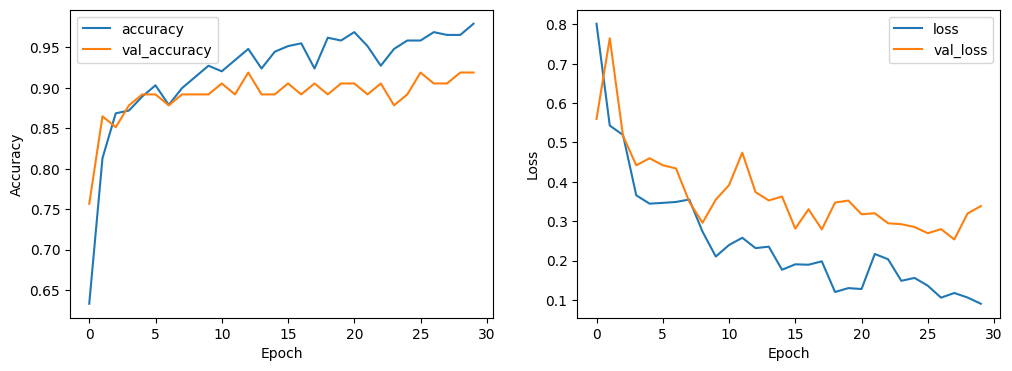
\includegraphics[width=0.5\textwidth]{training_eval_loss.png}}
\caption{Training and Evaluation Loss Curves}
\label{fig:loss_curves}
\end{figure}

\subsubsection*{Evaluation on Test data}
The model was evaluated on the test data, and the following results were obtained:

\begin{table}[htbp]
\caption{Classification Report YAMNet}
\begin{center}
\begin{tabular}{|c|c|c|c|}
\hline
\textbf{Class} & \textbf{Precision} & \textbf{Recall} & \textbf{F1-Score} \\
\hline
Cry & 1.00 & 1.00 & 1.00 \\
\hline
Scream & 1.00 & 0.82 & 0.90 \\
\hline
Speech & 0.85 & 1.00 & 0.92 \\
\hline
\textbf{Accuracy} & \multicolumn{3}{|c|}{0.94} \\
\hline
\textbf{Macro Avg} & 0.95 & 0.94 & 0.94 \\
\hline
\textbf{Weighted Avg} & 0.95 & 0.94 & 0.94 \\
\hline
\end{tabular}
\label{tab:classification_report_yamnet}
\end{center}
\end{table}

\begin{table}[htbp]
\caption{Confusion Matrix YAMNet}
\begin{center}
\begin{tabular}{|c|c|c|c|}
\hline
& \textbf{Cry} & \textbf{Scream} & \textbf{Speech} \\
\hline
Cry & 11 & 0 & 0 \\
\hline
Scream & 0 & 9 & 2 \\
\hline
Speech & 0 & 0 & 11 \\
\hline
\end{tabular}
\label{tab:confusion_matrix_yamnet}
\end{center}
\end{table}

\subsection{Wav2Vec2}
Wav2Vec2\cite{wav2vec2} is a pretrained model for speech recognition. It also can be used as feature extractor with 768-dimensional embeddings. I have tried two approaches:
\begin{itemize}
    \item Using the pretrained model as a feature extractor and training a custom MLP classifier on top of it.
    \item Fine-tuning the pretrained model on the dataset.
\end{itemize}

\subsubsection*{Model Training and Evaluation}
I have used the first approach as it gave better results. Fine-tuning the model took a long time and even after that results were not satisfactory. Maybe more epochs would be required, but that comes at the cost of important time and compute resources.
The extracted features were passed through a custom MLP classifier with following architecture:
\begin{table}[htbp]
\caption{Wav2Vec2-based MLP Classifier Architecture}
\begin{center}
\begin{tabular}{|c|c|c|}
\hline
\textbf{Layer (type)} & \textbf{Output Shape} & \textbf{Param \#} \\
\hline
Dense (ReLU) & (None, 256) & 262400 \\
\hline
Dense (Softmax) & (None, 3) & 771 \\
\hline
\end{tabular}
\label{tab:wav2vec2_mlp}
\end{center}
\end{table}

\begin{figure}[htbp]
\centerline{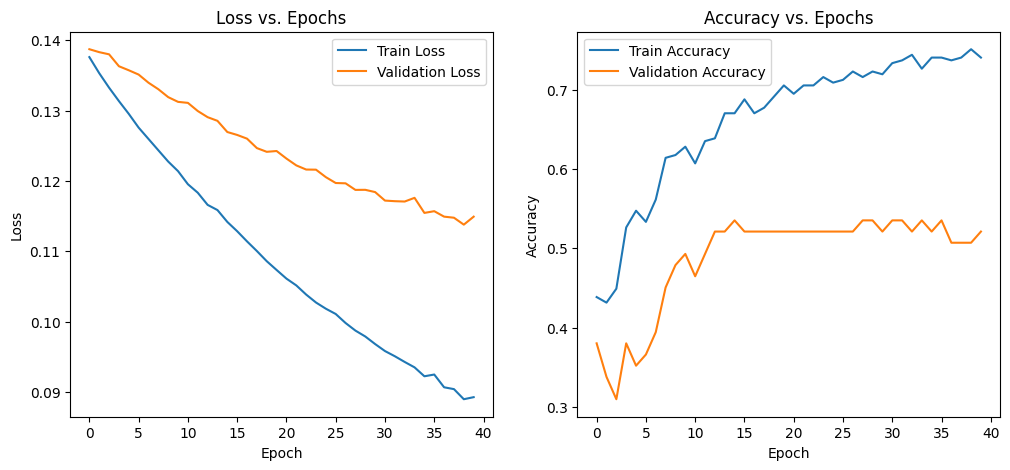
\includegraphics[width=0.5\textwidth]{wav2vec2_training_eval_loss.png}}
\caption{Training and Evaluation Loss Curves for Wav2Vec2-based MLP Classifier}
\label{fig:wav2vec2_loss_curves}
\end{figure}

\subsubsection*{Evaluation on Test data}
The model was evaluated on the test data, and the following results were obtained:
\begin{table}[htbp]
\caption{Classification Report Wav2Vec2}
\begin{center}
\begin{tabular}{|c|c|c|c|}
\hline
\textbf{Class} & \textbf{Precision} & \textbf{Recall} & \textbf{F1-Score} \\
\hline
Class 1 & 1.00 & 0.90 & 0.95 \\
\hline
Class 2 & 0.43 & 0.38 & 0.40 \\
\hline
Class 3 & 0.50 & 0.64 & 0.56 \\
\hline
\textbf{Accuracy} & \multicolumn{3}{|c|}{0.725} \\
\hline
\textbf{Macro Avg} & 0.64 & 0.64 & 0.64 \\
\hline
\end{tabular}
\label{tab:classification_report_wav2vec2}
\end{center}
\end{table}

\begin{table}[htbp]
\caption{Confusion Matrix Wav2Vec2}
\begin{center}
\begin{tabular}{|c|c|c|c|}
\hline
& \textbf{Cry} & \textbf{Scream} & \textbf{Speech} \\
\hline
Cry & 19 & 0 & 0 \\
\hline
Scream & 0 & 3 & 4 \\
\hline
Speech & 2 & 5 & 7 \\
\hline
\end{tabular}
\label{tab:confusion_matrix_wav2vec2}
\end{center}
\end{table}



\section{Ensemble Model}
An ensemble of YAMNet and Wav2Vec2 models was utilized to enhance robustness and improve overall performance. Three different ensemble techniques were explored:
\subsection{Ensemble Techniques}
I explored multiple ensemble learning techniques to enhance classification performance. Ensemble methods reduce variance and improve generalization. The following ensemble techniques were implemented and evaluated:
\subsubsection{Average}
In this technique, the probabilities predicted by each model are averaged to get the final prediction. This helps in smoothing out the predictions and reducing the variance.

\subsubsection{Weighted Average}
In this technique, the probabilities predicted by each model are weighted according to their performance on the validation set. The final prediction is obtained by averaging these weighted probabilities. This helps in giving more importance to the better performing model.

\subsubsection{Hard Voting}
In this technique, the final prediction is obtained by taking the majority vote of the predictions made by each model. This helps in reducing the bias and making the final prediction more robust.

\subsubsection*{Evaluation on Test data}
The ensemble model was evaluated on the test data, and the following results were obtained:

\begin{table}[htbp]
\caption{Classification Report Ensemble Model (Simple Average)}
\begin{center}
\begin{tabular}{|c|c|c|c|}
\hline
\textbf{Class} & \textbf{Precision} & \textbf{Recall} & \textbf{F1-Score} \\
\hline
Cry & 0.92 & 1.00 & 0.96 \\
\hline
Scream & 1.00 & 0.92 & 0.96 \\
\hline
Speech & 1.00 & 1.00 & 1.00 \\
\hline
\textbf{Accuracy} & \multicolumn{3}{|c|}{0.97} \\
\hline
\textbf{Macro Avg} & 0.97 & 0.97 & 0.97 \\
\hline
\textbf{Weighted Avg} & 0.97 & 0.97 & 0.97 \\
\hline
\end{tabular}
\label{tab:classification_report_ensemble}
\end{center}
\end{table}

\begin{table}[htbp]
\caption{Confusion Matrix Ensemble Model (Simple Average)}
\begin{center}
\begin{tabular}{|c|c|c|c|}
\hline
& \textbf{Cry} & \textbf{Scream} & \textbf{Speech} \\
\hline
Cry & 12 & 0 & 0 \\
\hline
Scream & 1 & 11 & 0 \\
\hline
Speech & 0 & 0 & 12 \\
\hline
\end{tabular}
\label{tab:confusion_matrix_ensemble}
\end{center}
\end{table}

\begin{table}[htbp]
\caption{Classification Report Ensemble Model (Hard Voting)}
\begin{center}
\begin{tabular}{|c|c|c|c|}
\hline
\textbf{Class} & \textbf{Precision} & \textbf{Recall} & \textbf{F1-Score} \\
\hline
Cry & 0.75 & 1.00 & 0.86 \\
\hline
Scream & 0.69 & 0.75 & 0.72 \\
\hline
Speech & 1.00 & 0.58 & 0.74 \\
\hline
\textbf{Accuracy} & \multicolumn{3}{|c|}{0.78} \\
\hline
\textbf{Macro Avg} & 0.81 & 0.78 & 0.77 \\
\hline
\textbf{Weighted Avg} & 0.81 & 0.78 & 0.77 \\
\hline
\end{tabular}
\label{tab:classification_report_hard_voting}
\end{center}
\end{table}

\begin{table}[htbp]
\caption{Confusion Matrix Ensemble Model (Hard Voting)}
\begin{center}
\begin{tabular}{|c|c|c|c|}
\hline
& \textbf{Cry} & \textbf{Scream} & \textbf{Speech} \\
\hline
Cry & 12 & 0 & 0 \\
\hline
Scream & 3 & 9 & 0 \\
\hline
Speech & 1 & 4 & 7 \\
\hline
\end{tabular}
\label{tab:confusion_matrix_hard_voting}
\end{center}
\end{table}

\begin{table}[htbp]
\caption{Classification Report Ensemble Model (Weighted Average)}
\begin{center}
\begin{tabular}{|c|c|c|c|}
\hline
\textbf{Class} & \textbf{Precision} & \textbf{Recall} & \textbf{F1-Score} \\
\hline
Cry & 0.92 & 1.00 & 0.96 \\
\hline
Scream & 1.00 & 0.92 & 0.96 \\
\hline
Speech & 1.00 & 1.00 & 1.00 \\
\hline
\textbf{Accuracy} & \multicolumn{3}{|c|}{0.97} \\
\hline
\textbf{Macro Avg} & 0.97 & 0.97 & 0.97 \\
\hline
\textbf{Weighted Avg} & 0.97 & 0.97 & 0.97 \\
\hline
\end{tabular}
\label{tab:classification_report_weighted_average}
\end{center}
\end{table}

\begin{table}[htbp]
\caption{Confusion Matrix Ensemble Model (Weighted Average)}
\begin{center}
\begin{tabular}{|c|c|c|c|}
\hline
& \textbf{Cry} & \textbf{Scream} & \textbf{Speech} \\
\hline
Cry & 12 & 0 & 0 \\
\hline
Scream & 1 & 11 & 0 \\
\hline
Speech & 0 & 0 & 12 \\
\hline
\end{tabular}
\label{tab:confusion_matrix_weighted_average}
\end{center}
\end{table}

\subsection{Loss Function}
The loss function used for training both the models was categorical cross-entropy. This is a standard loss function for multi-class classification problems. It calculates the cross-entropy loss between the predicted probabilities and the true labels.
\begin{equation}
    L(y, \hat{y}) = -\sum_{i} y_i \log(\hat{y}_i)
\end{equation}
where $y$ is the true label, $\hat{y}$ is the predicted probability, and $i$ is the class index. 

While training the model with best validation accuracy was saved. And later these weights were used to evaluate the model on test data.

\section{Deployment with Temporal}
The ensemble model was deployed using Temporal and Streamlit for UI.

The Streamlit UI has two sections:
\begin{itemize}
    \item \textbf{Upload Audio:} Users can upload an audio file to classify it as either a cry, scream, or speech.
    \item \textbf{Record Audio:} Users can record audio using their microphone and classify it as either a cry, scream, or speech.
\end{itemize}

The Temporal workflow consists of the following steps:
\begin{itemize}
    \item \textbf{Preprocess Audio:} If the audio is recorded, it is first saved as a .wav file. Now, the saved .wav files are preprocessed to convert them to 16kHz mono channel audio files. This allows real time audio processing, User recorded audio is saved and preprocessed.
    \item \textbf{Classification} The preprocessed audio files are then passed through the ensemble model to classify them as either a cry, scream, or speech.
    \item \textbf{Display Results:} The classification results with confidence are displayed to the user in the Streamlit UI.
    \item \textbf{Save Results:} The classification results are saved in a .json file for future reference.
\end{itemize}

As mentioned above, during inference the extraction of both model doens't require fixed length audio files. So, given any audio file, the features are extracted and passes to respective MLP classifier. Which in turn is used by ensemble to predict the label with a confidence score.

\begin{figure}[htbp]
\centerline{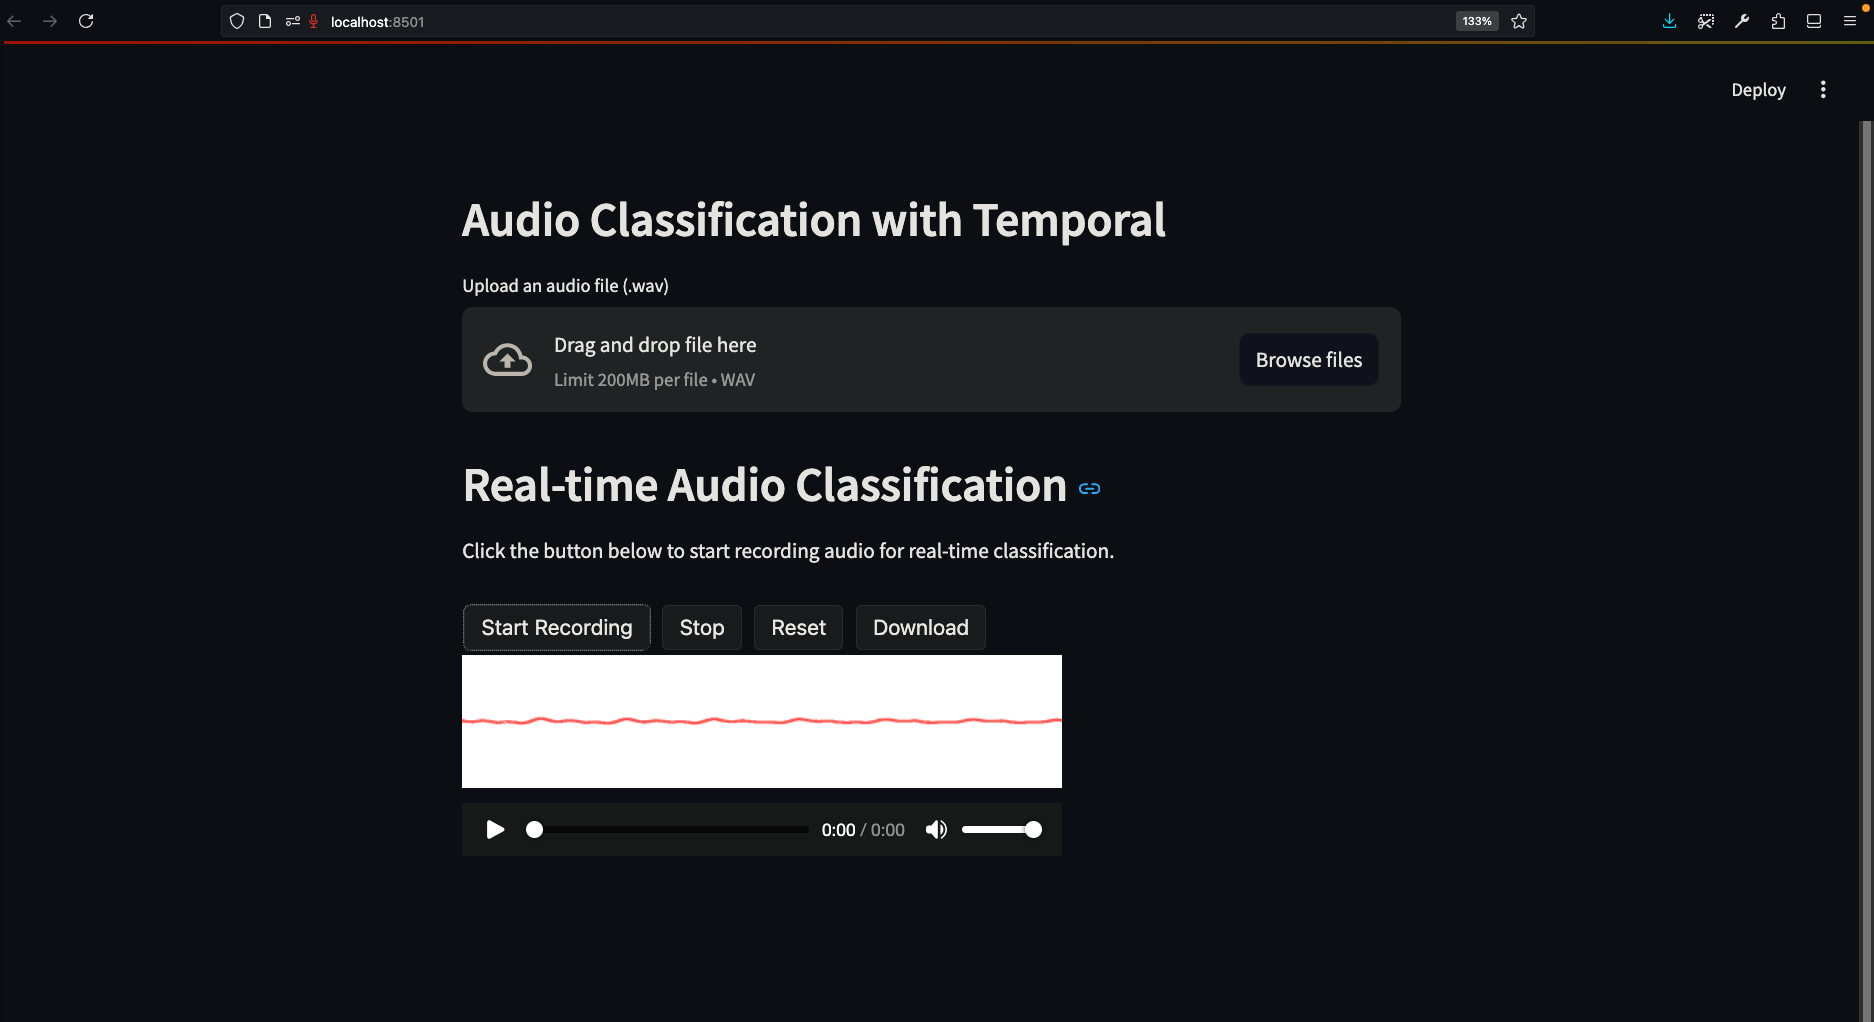
\includegraphics[width=0.5\textwidth]{streamlit.png}}
\caption{Streamlit UI for Audio Classification}
\label{fig:streamlit_ui}
\end{figure}

\begin{figure}[htbp]
\centerline{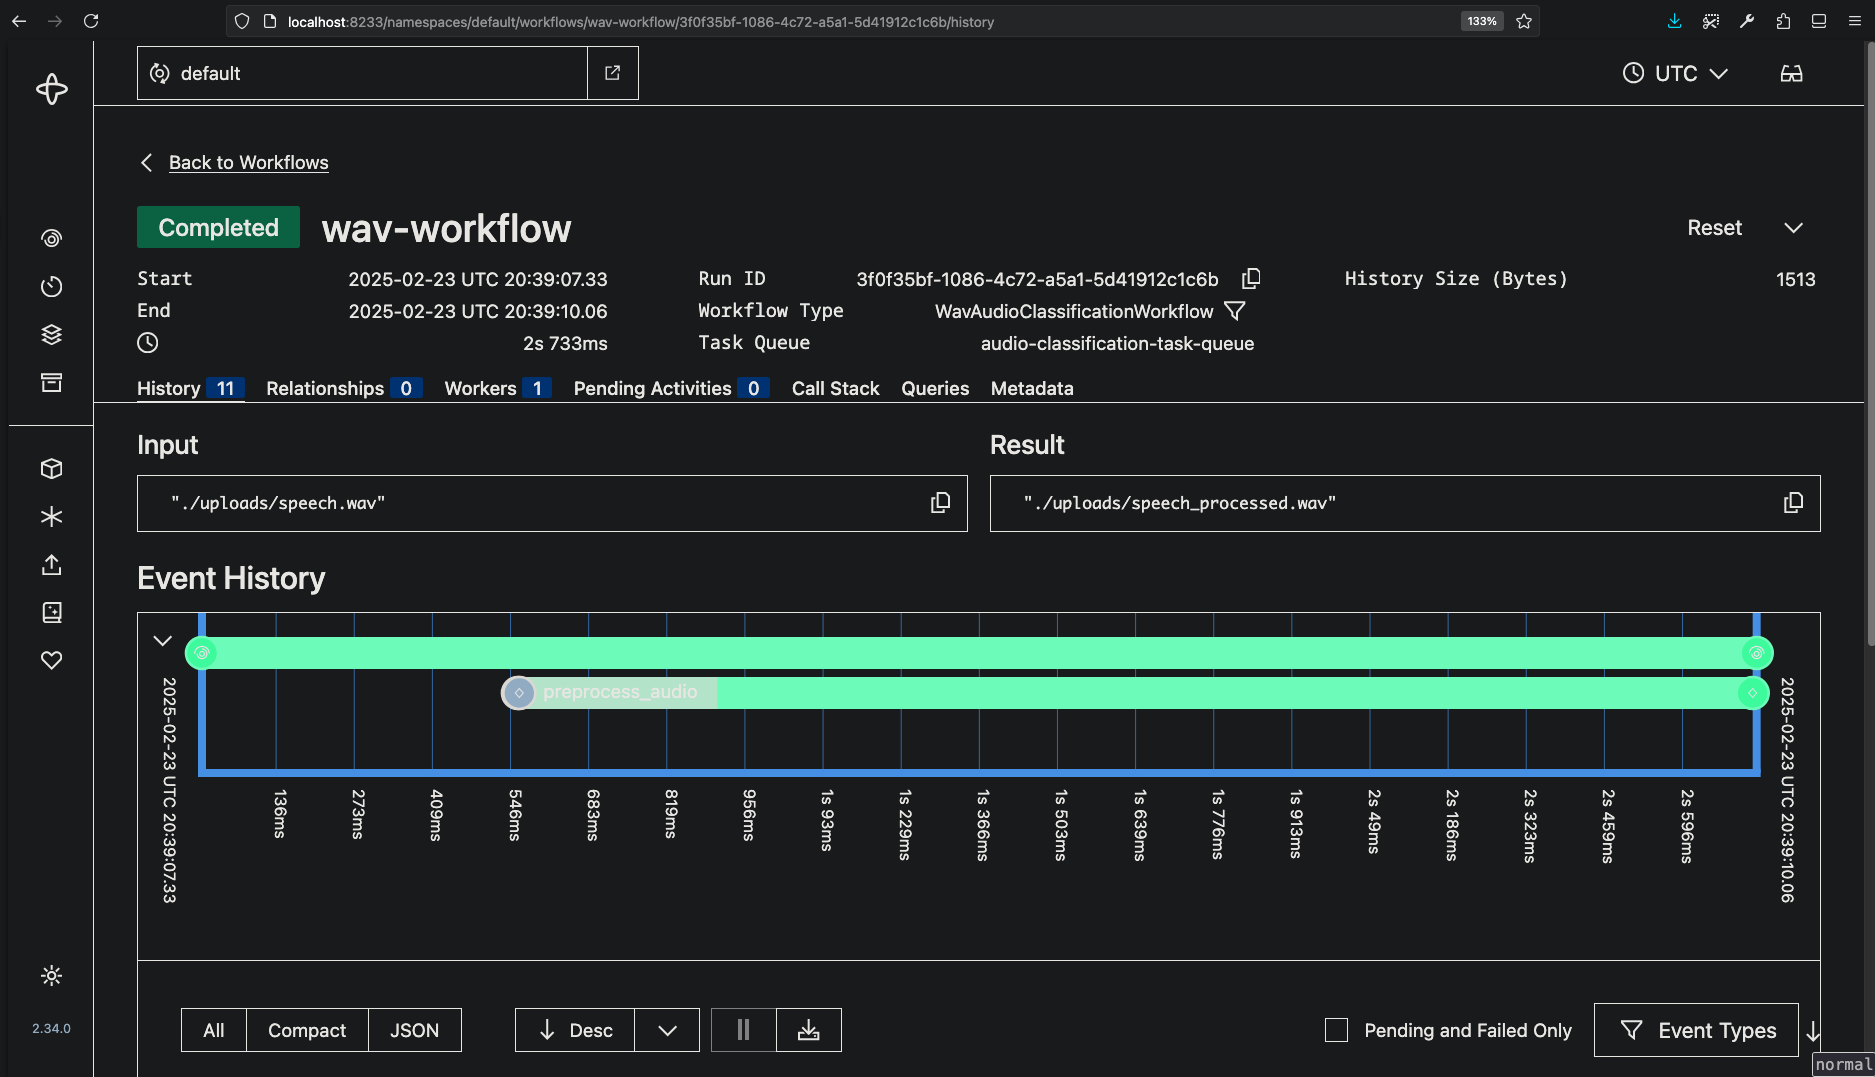
\includegraphics[width=0.5\textwidth]{temporal.png}}
\caption{Temporal UI for Workflow Management}
\label{fig:temporal_ui}
\end{figure}



\begin{thebibliography}{00}
    \bibitem{dataset1} Rosita, Yesy Diah (2020), “Infant's Cry Sound”, Mendeley Data, V1, doi: 10.17632/hbppd883sd.1
    \bibitem{dataset2} Kaggle: Human Screaming Detection Dataset, \url{https://www.kaggle.com/datasets/whats2000/human-screaming-detection-dataset}.
    \bibitem{dataset3} AudioSet: Child speech, kid speaking, \url{https://research.google.com/audioset/dataset/child_speech_kid_speaking.html}.
    \bibitem{data-augmentation} J. Salamon and J. P. Bello, "Deep Convolutional Neural Networks and Data Augmentation for Environmental Sound Classification," in IEEE Signal Processing Letters, vol. 24, no. 3, pp. 279-283, March 2017, doi: 10.1109/LSP.2017.2657381. 
    \bibitem{yamnet} YAMNet model, \url{https://tfhub.dev/google/yamnet/1}. 
    \bibitem{wav2vec2} Baevski, Alexei, et al. "wav2vec 2.0: A Framework for Self-Supervised Learning of Speech Representations." arXiv preprint arXiv:2006.11477 (2020). \url{https://arxiv.org/abs/2006.11477}.
\end{thebibliography}
\vspace{12pt}

\end{document}
